\documentclass[11pt,a4paper]{jsarticle}
%
\usepackage{amsmath,amssymb}
\usepackage{bm}
\usepackage{graphicx}
\usepackage{ascmac}
\usepackage{atbegshi}
\usepackage{geometry} % 追加: 余白を一時的に0にするため
\usepackage{listings} % ソースコード表示のために追加
%ここからソースコードの表示に関する設定
\lstset{
  basicstyle={\ttfamily},
  identifierstyle={\small},
  commentstyle={\smallitshape},
  keywordstyle={\small\bfseries},
  ndkeywordstyle={\small},
  stringstyle={\small\ttfamily},
  frame={tb},
  breaklines=true,
  columns=[l]{fullflexible},
  numbers=left,
  xrightmargin=0zw,
  xleftmargin=3zw,
  numberstyle={\scriptsize},
  stepnumber=1,
  numbersep=1zw,
  lineskip=-0.5ex
}
\renewcommand{\lstlistingname}{ソースコード} % キャプションを「ソースコード」に変更
%ここまでソースコードの表示に関する設定
\newcommand{\myPdfAuthor}{平田爽馬/HIRATA,Soma}
\newcommand{\myPdfTitle}{Webセキュリティ実験}
\AtBeginShipoutFirst{\special{pdf:tounicode EUC-UCS2}} % pLaTeXの内部漢字コードがEUCの場合
\AtBeginDvi{\special{pdf:docinfo <<
 /Author   (\myPdfAuthor)
 /Title    (\myPdfTitle)>>}}
%
\setlength{\textwidth}{\fullwidth}
\setlength{\textheight}{40\baselineskip}
\addtolength{\textheight}{\topskip}
\setlength{\voffset}{-0.2in}
\setlength{\topmargin}{0pt}
\setlength{\headheight}{0pt}
\setlength{\headsep}{0pt}
%
\newcommand{\divergence}{\mathrm{div}\,}  %ダイバージェンス
\newcommand{\grad}{\mathrm{grad}\,}  %グラディエント
\newcommand{\rot}{\mathrm{rot}\,}  %ローテーション
%
\title{\myPdfTitle}
\author{5E25番 平田爽馬}
\date{}
\begin{document}
%\maketitle%タイトルを挿入したくない場合は,消す
%
%
\section{目的}
現代ではゲームサーバ・通販サイトなどのサービスを,ネットワーク知識がなくても容易に解説できるまでになっている.
しかし,これらのサービスには脆弱性を意図せず含んでしまう場合があり,アカウント情報が盗まれるなどの被害が出る可能性がある.
そのため,本実験では実際に脆弱性を体験し,適切な対策を考察することを目的とする.

\section{SQLインジェクションによるデータベースの不正ログイン}
\subsection*{データベース}
データベースは決まった条件で整理されたデータの集まりであり,コンピュータ上で大量のデータを効率よく利用するために使用される.
図\ref{fig1}にデータベースの例を示す.データベースはテーブル(表)を単位として構成され,カラム(列),レコード(行),フィールド(セル)の要素を持つ.
カラムにはデータの属性を示し,レコードは1件分のデータのまとまりである.フィールドには,実際の個々のデータが格納される.

\begin{figure}[htbp]
\centering
\includegraphics[width=90mm]{./fig/fig1.eps}
\caption{データベースの名称}
\label{fig1}
\end{figure}

\subsection*{SQLインジェクション}
SQL(StructuredQueryLanguage)とは,データベースに対してデータの検索・追加・更新・削除といった操作を行うための言語である.
SQLインジェクションは,図\ref{fig2}のようにアプリケーションがデータベースとやり取りを行う際に,悪意のあるSQLコードを挿入することで,不正な操作を実行させる攻撃手法である.
この攻撃により,攻撃者はデータベース内の情報を不正に取得,改ざん,削除することが可能となる.

\begin{figure}[htbp]
\centering
\includegraphics[width=90mm]{./fig/fig2.eps}
\caption{SQLインジェクションの例}
\label{fig2}
\end{figure}

\subsection*{実験1:XAMMPを用いたGET・POSTの動作確認}
本実験では,XAMMPを用いて仮想的なサーバを立ち上げて実験を行う.
XAMMPはウェブ開発に必要なソフトApache,MariaDB(MySQL),PHP,Perlを一括でインストールできるパッケージソフトウェアである.
ローカル環境で動作するため,既存のシステムに影響を与えず検証が可能である.\\\\
以下のリンクより,XAMMPをインストールする.\\
\fbox{https://www.apachefriends.org/index.html}\\\\
図\ref{fig3}のように,Startボタンを押して→Stopに切り替わった後,Statusマークが緑色になると準備が完了となる.

\begin{figure}[htbp]
\centering
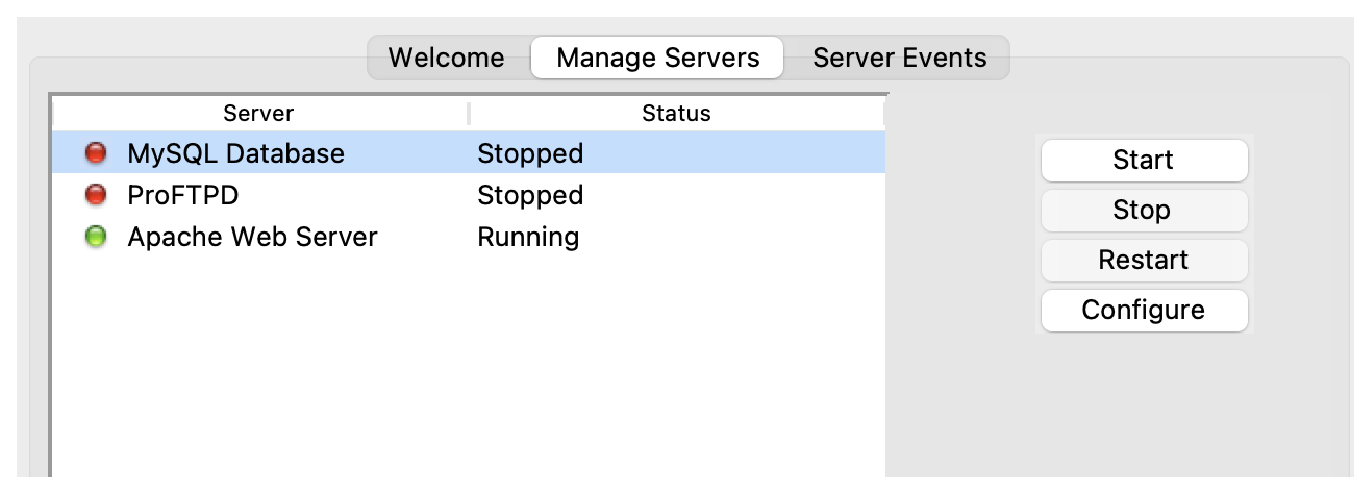
\includegraphics[width=85mm]{./fig/fig3.eps}
\caption{XAMMPの起動画面}
\label{fig3}
\end{figure}

XAMMPインストール後,xammp/htdocsフォルダが生成される.\\
(デフォルトはC:/xammp/htdocs)\\
このフォルダにHTML,PHPファイルなどを置くことで,ブラウザ上からアクセスできるようになる.\\\\
(例)\\
C:/xammp/htdocs/index.htmlを置く→ブラウザでhttp://localhost/index.htmlで動作確認できる.

\subsubsection*{課題1}
login.htmlおよびsession.phpを作成し,login.html上でGET・POSTの動作の違いが何か,URL欄を見て確認する.
また,GET・POSTの使い分けは何か調査し,まとめる.
\newpage
login.htmlをソースコード\ref{code1}に示す.

\begin{lstlisting}[caption=login.html, label=code1]
<html>
    <head>
        <title>Login Page</title>
    </head>
    <body>
        <h1>Login</h1>
        <form action="login.php" method="post">
            user:<input type="text" name="username" value=""><br />
            password:<input type="password" name="password" required><br />
            <input type="submit" name="login" value="Login">
        </form>
    </body>
</html>
\end{lstlisting}

session.phpをソースコード\ref{code2}に示す.
\begin{lstlisting}[caption=session.php, label=code2]
<?php
session_start();

$_SESSION["loginname"] = $_POST["username"];
$_SESSION["pass"] = $_POST["pass"];

if($_SESSION["loginname"] != "hoge" || $_SESSION["pass"] != "pass"){
?>
Login Failed<br />

<?php

 exit;

}

if(isset($_POST["username"])) setcookie("username", $_POST["username"], time());
?>
Login Succeeded<br />
\end{lstlisting}



\subsection{目的}
...
...

\subsubsection{構成}

\section{初めに}
\subsection{背景}
...
...
sw

\subsection{目的}
...
...

\subsubsection{構成}
こんにちは
dchweqodejqcフェくぃうfdcbwdw\\ %強制改行
\raise0.2ex\hbox{\textcircled{\scriptsize{2}}}\\

平田は自身のLaTeX講座の集大成として学習ガイドを執筆した\cite{hajime}.

\begin{thebibliography}{99}
\bibitem{hajime} 塚原壮平, 「初めてのLaTeX講座」, 九大新書, 2023.
\bibitem{soryu} 塚原壮平, 「素粒子物理学入門」, きゅうり図書, 2023.
\end{thebibliography}
%
\end{document}